\section{Real-time Implementation}

% agenda maybe changed a bit.

% fga, throughput and latency, accuracy
% benchmark, throughput
% demo or a picture.

\begin{frame}
    \frametitle{Task Based Signal Processing System}

    \begin{columns}
      \begin{column}{0.515\textwidth}
        
        \begin{itemize}
          \item Using a task based digital signal processing system at the receiver 
          \begin{itemize}
              \item Each function maps to an individual task. 
              \item Tasks are processed in parallel if no data dependency occurs.             
             
          \end{itemize} 
          \item Different aspects of the algorithm are mapped in 
          a pipelined, parallel task processing architecture via Threading Building Blocks~\cite{Michael_19}. 


        \end{itemize}

      \end{column} 

    \begin{column}{0.46\textwidth} 

        \begin{center}
          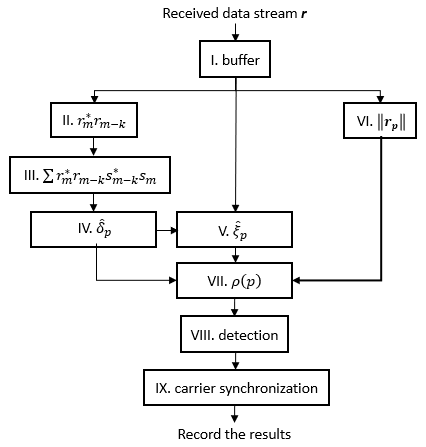
\includegraphics[width=1.0\linewidth]{SDR_receiver_new_slides.png}
        \end{center}
      
      \end{column}
    \end{columns}

    % \begin{figure}
    %     \centering
    %     \begin{minipage}{.5\textwidth}
    %       \centering
    %       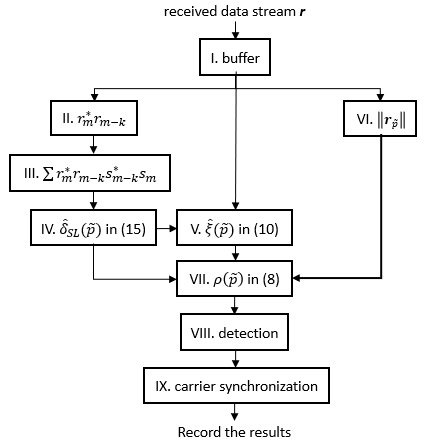
\includegraphics[width=.5\linewidth]{SDR_receiver_new.png}
    %     \end{minipage}%
    %     \begin{minipage}{.5\textwidth}
    %       \centering
    %       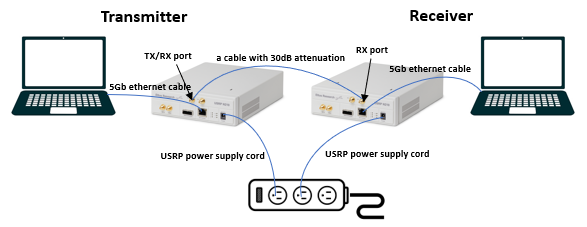
\includegraphics[width=.8\linewidth]{SDR_signal_transmission_path.png}
    %     \end{minipage}
    % \end{figure}

    % \begin{itemize}
    %     \item Different aspects of our algorithm are mapped to logical nodes in a pipelined, parallel processing architecture using Threading Building Blocks (TBB).
    %     \item The signals are transmitted and received between two universal software radio peripherals (USRP) connected by 5 Gb/s Ethernet cables to
    %     laptops.
    %     \item Accuracy, throughput and latency (the time when the first joint detection and estimation are finished) are considered. 
    % \end{itemize}
  \end{frame}


  \begin{frame}
    \frametitle{Software-defined Radio}
    \begin{center}
      \includegraphics[width=.8\textwidth]{SDR_real.jpeg}
    \end{center}

  \end{frame} 


  \begin{frame}
    \frametitle{Flow Graph Analyzer~\cite{Intel_Corporation}: Latency and Throughput}

    % need more explain on how FGA works.

    \begin{figure}
        \centering
          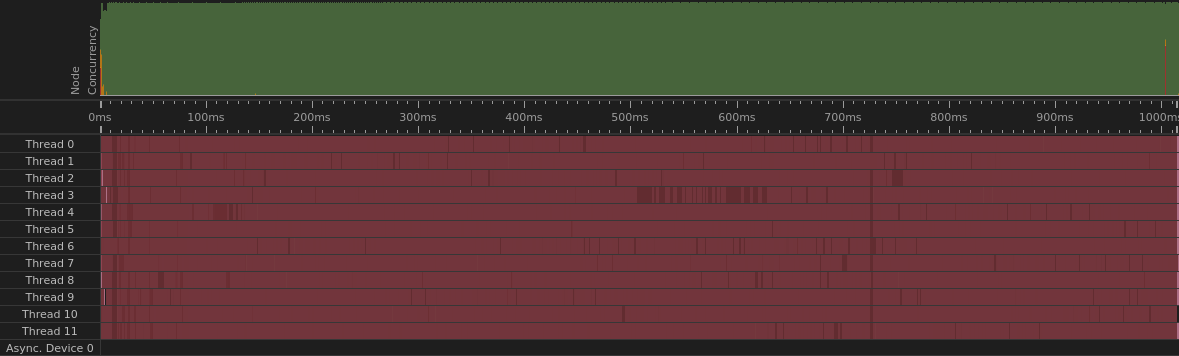
\includegraphics[width=.62\linewidth]{fga_throughput.png}
    \end{figure}

    \begin{figure}
      \centering
        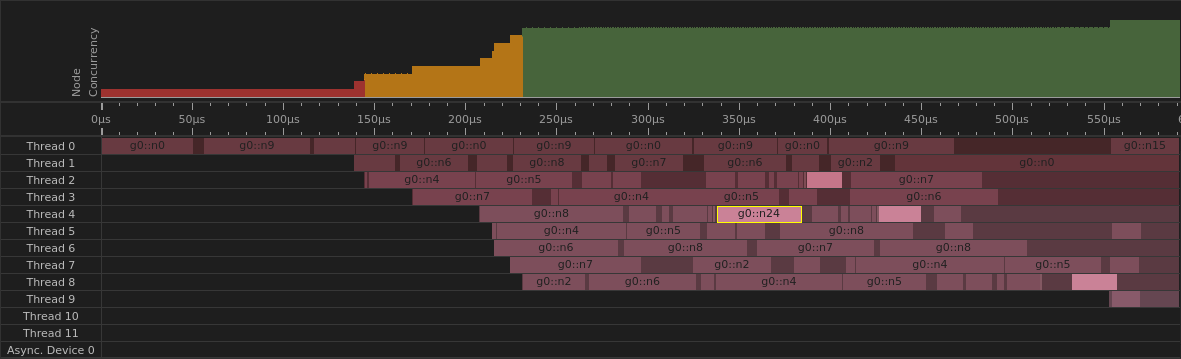
\includegraphics[width=.62\linewidth]{fga_latency.png}
  \end{figure}

    \begin{itemize}
        \item The top graph shows that the task based implementation
          exhibits high parallelism; all cores are used.
          \begin{itemize}
          \item The throughput is approximately
            $ \SI[per-mode=symbol]{28.74}{\mega\sample\per\second}$.
          \end{itemize}
        \item By zooming in on the start of processing, the latency (finish time of the first burst) is observed around $ \SI[per-mode=symbol]{383.7}{\micro\second}$.

    \end{itemize}
  \end{frame}


  \begin{frame}
    \frametitle{Google Benchmark: Task Duration Measurement}

    \begin{figure}
        \centering
        \begin{table}[t]
          \tiny
          \centering % used for centering table
          \begin{tabular}{c c c c} % centered columns (4 columns)
          \hline\hline %inserts double horizontal lines
          Node name & Time (ns) & CPU (ns) & Iterations \\ [0.5ex] % inserts table
          %heading
          \hline % inserts single horizontal line
          I. Buffer  & 3487 & 3487 & 206840 \\ % inserting body of the table
          II. $r_m^*r_{m-k}$  & 3530 & 3530 & 198687 \\
          III. $r_m^*r_{m-k}s_{m-k}^*s_m$ & 49290 & 49289 & 13958 \\
          IV. $\hat{\delta}_{SL}^{(1)}$ & 53219 & 53217 & 12180 \\
          V. $\hat{\xi}$ & 65397 & 65388 & 15312 \\
          VI. $||\bm{r}||$ & 13130 & 13129 & 52026 \\ % [1ex] adds vertical space
          VII. $\rho(p)$ & 7278 & 7278 & 92031 \\
          VIII. detection & 5521 & 5521 & 123079 \\
          IX. carrier synchronization & 46855 & 46851 & 14867  \\ [1ex]
          \hline
          \end{tabular}
          \label{table:BM_function_nodes} % is used to refer this table in the text
        \end{table}   
    \end{figure}

    \begin{itemize}
       \item Benchmark each task of proposed algorithm
         ($\SI{2048}{\sample}$ input):
       \begin{itemize}
        \item measure the throughput that each task can achieve
        \item identify the task with the longest duration for
          potential increase of throughput of the entire system
       \end{itemize}
       \item The throughput is bounded by slowest block, $\SI{2048}{\sample}/\SI{65397}{\nano\second}  \approx \SI[per-mode=symbol]{31.32}{\mega\sample\per\second}$.
    \end{itemize}
  \end{frame}

 


  \begin{frame}
    \frametitle{Summary and Future Work}
    \begin{itemize}
      \item A family of algorithms for joint detection and carrier synchronization for LPI/LPD communications was presented.
      \begin{itemize}
        \item The algorithm is designed for low complexity while achieving good performance over a wide range of SNR.
      \end{itemize}
      \item The real-time practicality of the algorithm is validated via a software-defined radio platform.
      \begin{itemize}
        \item Different aspects of algorithm are mapped in a highly pipelined and parallel task architecture.
      \end{itemize}
      \item Extend the proposed algorithm for dispersive channels.
      \item Package the C++ code of real-time implementation as the open source distribution.
    \end{itemize}
      
  \end{frame} 